\documentclass[a4paper, 11pt]{article}
\usepackage{comment} % enables the use of multi-line comments (\ifx \fi) 

\usepackage{fullpage} % changes the margin
\usepackage{longtable}
\usepackage{graphicx}
\usepackage{fancyvrb,xcolor}
\usepackage{listings}
\usepackage{color}
\usepackage[margin=3cm]{geometry}
\usepackage{relsize}
\definecolor{dkgreen}{rgb}{0,0.6,0}
\definecolor{gray}{rgb}{0.5,0.5,0.5}
\definecolor{mauve}{rgb}{0.58,0,0.82}
\definecolor{LightCyan}{rgb}{0.88,1,1}
\usepackage{float}
\usepackage{caption}
\DeclareCaptionFont{white}{\color{white}}
\DeclareCaptionFormat{listing}{\colorbox{gray}{\parbox{\textwidth}{#1#2#3}}}
\captionsetup[lstlisting]{format=listing,labelfont=white,textfont=white}
\newcommand{\bigqm}[1][1]{\text{\larger[#1]{\textbf{?}}}}
\lstset{
  language=Java,
  aboveskip=3mm,
  belowskip=3mm,
  showstringspaces=false,
  columns=flexible,
  basicstyle={\small\ttfamily},
  numbers=none,
  numberstyle=\tiny\color{gray},
  keywordstyle=\color{blue},
  commentstyle=\color{dkgreen},
  stringstyle=\color{mauve},
  breaklines=true,
  breakatwhitespace=true,
  tabsize=3
}
\graphicspath{ {images/} }

\begin{document}
%Header-Make sure you update this information!!!!
\noindent
\large\textbf{Assignment 2} \hfill \textbf{Hussam Hallak} \\
\normalsize CS834, Information Retrieval, Fall 2017\hfill CS Master's Student \\
Old Dominion University, Computer Science Dept \hfill Prof: Dr. Nelson 

\section*{Question 1:}
Exercise 4.3: 

Try to estimate the number of web pages indexed by two different search engines using the technique described in this chapter. Compare the size estimates from a range of queries and discuss the consistency (or lack of it) of these estimates.

\subsection*{Answer:}
I have chosen Google and Bing search engines. The technique described in this chapter uses the formula:

$$
N=\frac{f_a \times f_b}{f_{ab}}
$$

Where:

$a$ and $b$ are the independent terms

$N$ is the estimated total number of indexed pages

$f_a$ is the number of pages containing the term $a$

$f_b$ is the number of pages containing the term $b$

$f_{ab}$ is the number of pages containing both $a$ and $b$

\paragraph{•}
The two terms in the query need to be as independent as possible, so I have chosen the following queries:

1. Diesel Memory

2. Hairy Phone

3. Computer Manifold

4. Electronic Lumber

\paragraph{1. Diesel Memory:}
I ran the first query ``Diesel Memory'' and found the following:

A. Google:

\pagebreak
Google found about 207,000,000 results for the term ``Diesel''.
\begin{figure}[h]
\caption{Query: Diesel, Search Engine: Google}
\centering
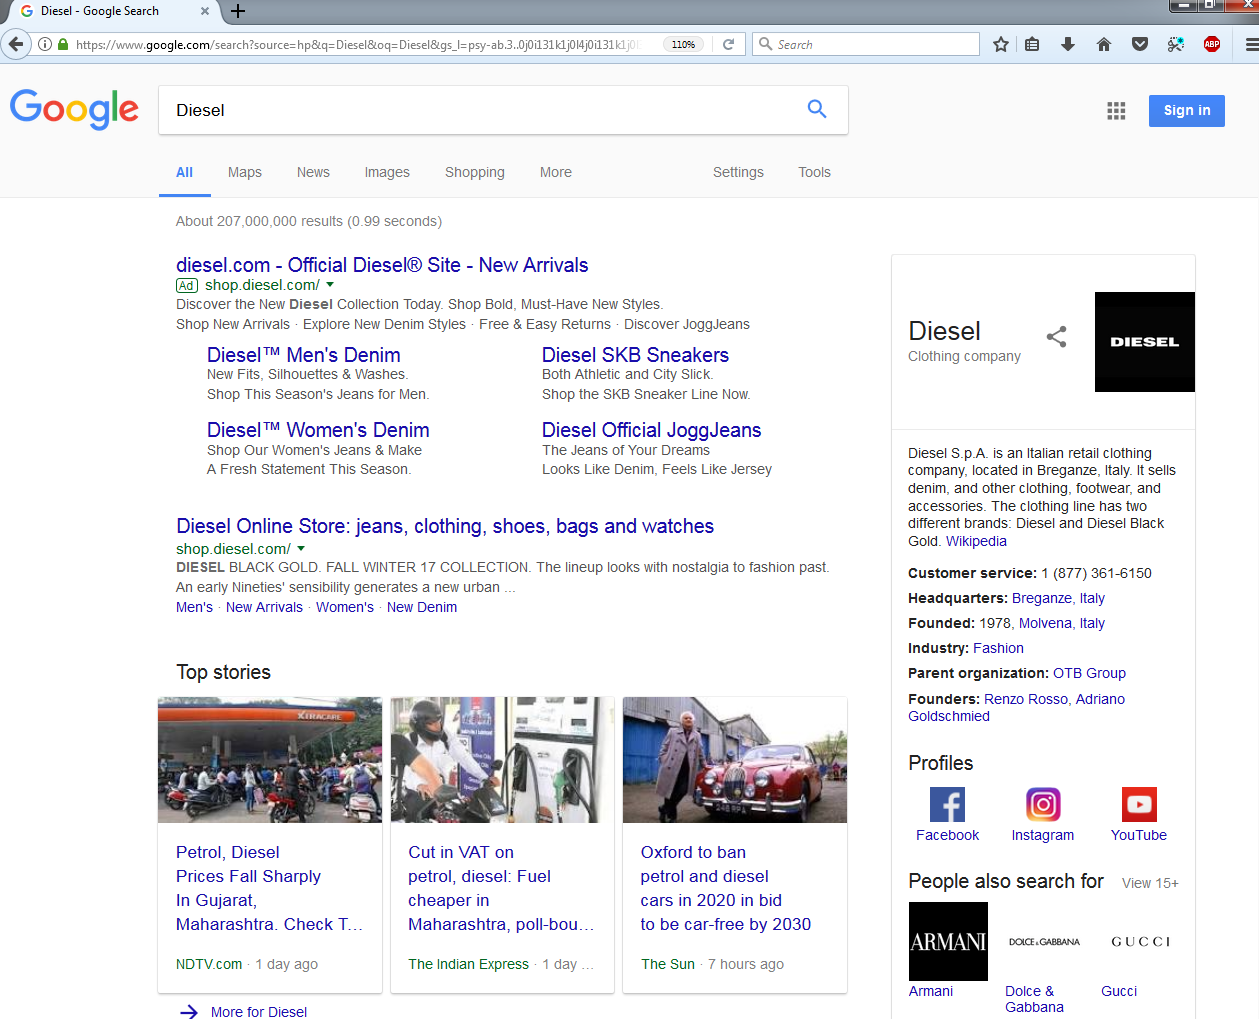
\includegraphics[scale=0.4]{Q1/DieselGoogle.png}
\end{figure}

\pagebreak
Google found about 377,000,000 results for the term ``Memory''.
\begin{figure}[h]
\caption{Query: Memory, Search Engine: Google}
\centering
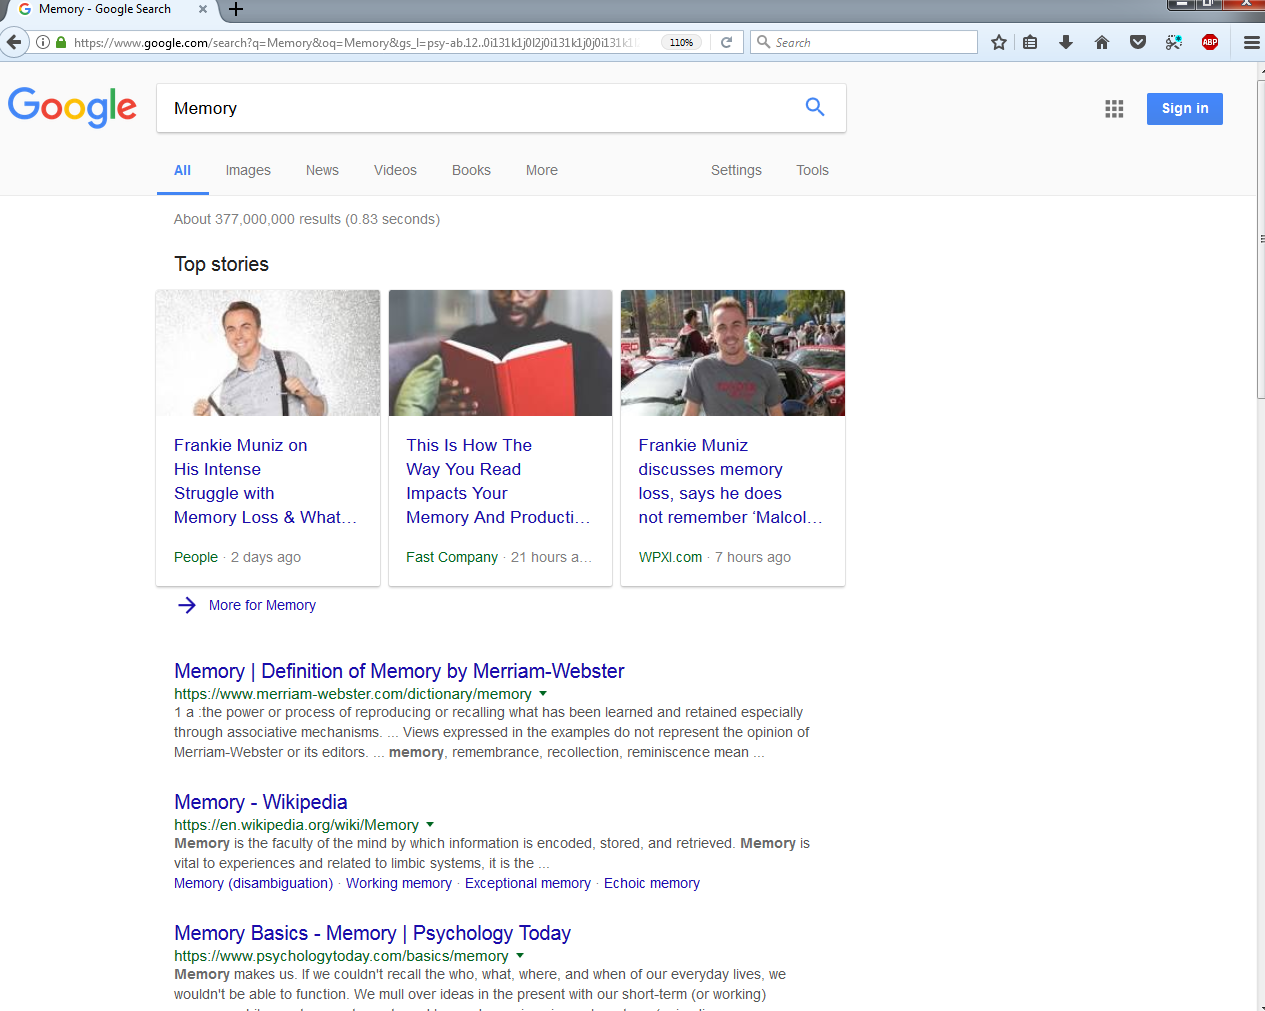
\includegraphics[scale=0.4]{Q1/MemoryGoogle.png}
\end{figure}

\pagebreak
Google found about 36,900,000 results for the query ``Diesel Memory''.
\begin{figure}[h]
\caption{Query: Diesel Memory, Search Engine: Google}
\centering
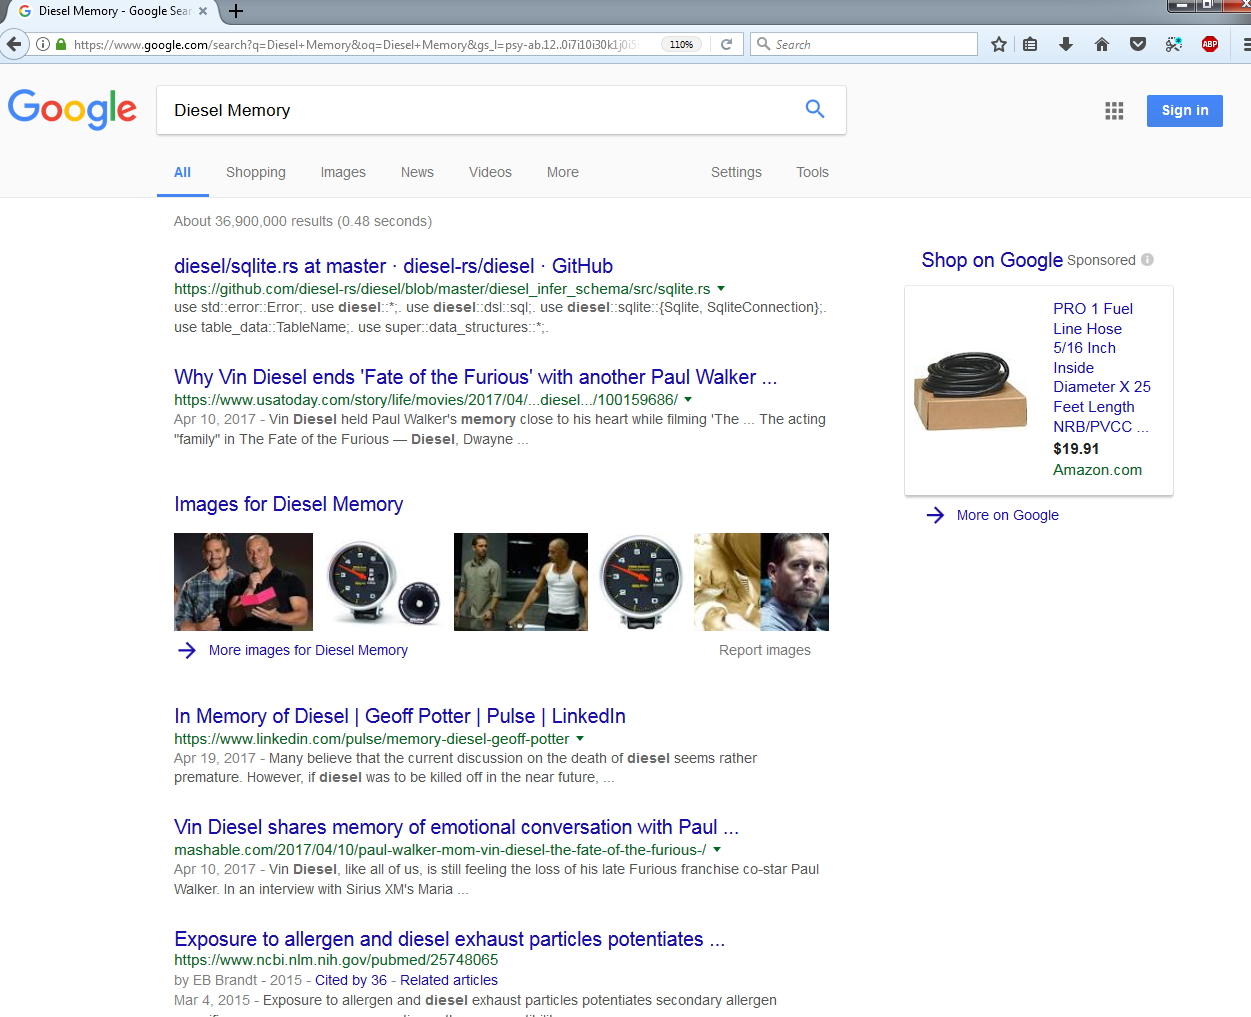
\includegraphics[scale=0.4]{Q1/DieselMemoryGoogle.png}
\end{figure}

Plugging the results in the formula gives the following:

$$N_{google} = \frac{207,000,000 \times 377,000,000}{36,900,000} = 2114878048.780488 \approx 2114878049
$$


\pagebreak

B. Bing:

Bing found about 183,000,000 results for the term ``Diesel''.
\begin{figure}[h]
\caption{Query: Diesel, Search Engine: Bing}
\centering
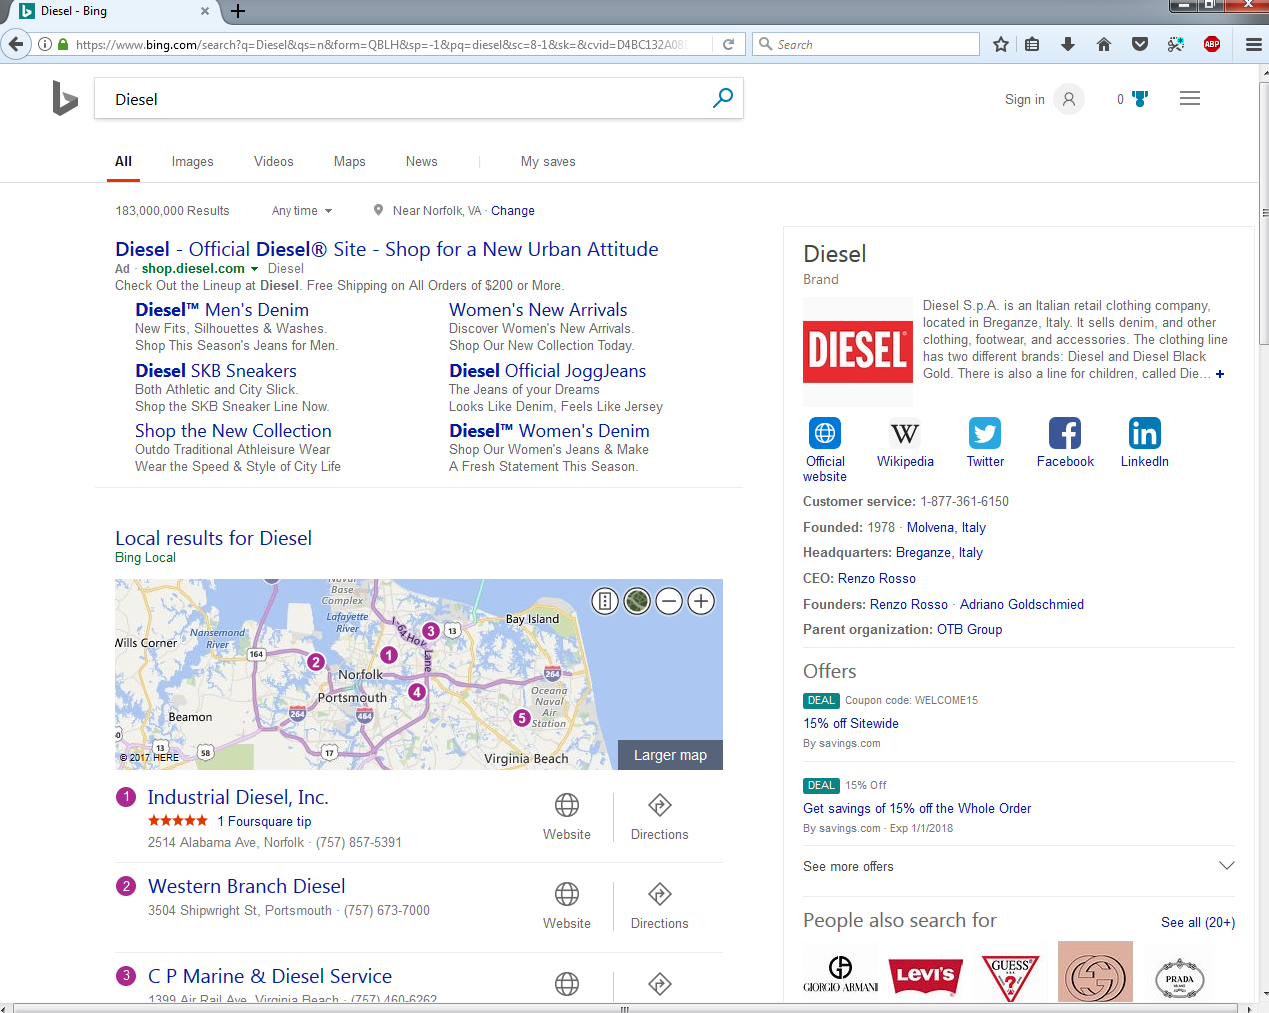
\includegraphics[scale=0.4]{Q1/DieselBing.png}
\end{figure}

\pagebreak
Bing found about 167,000,000 results for the term ``Memory''.
\begin{figure}[h]
\caption{Query: Memory, Search Engine: Bing}
\centering
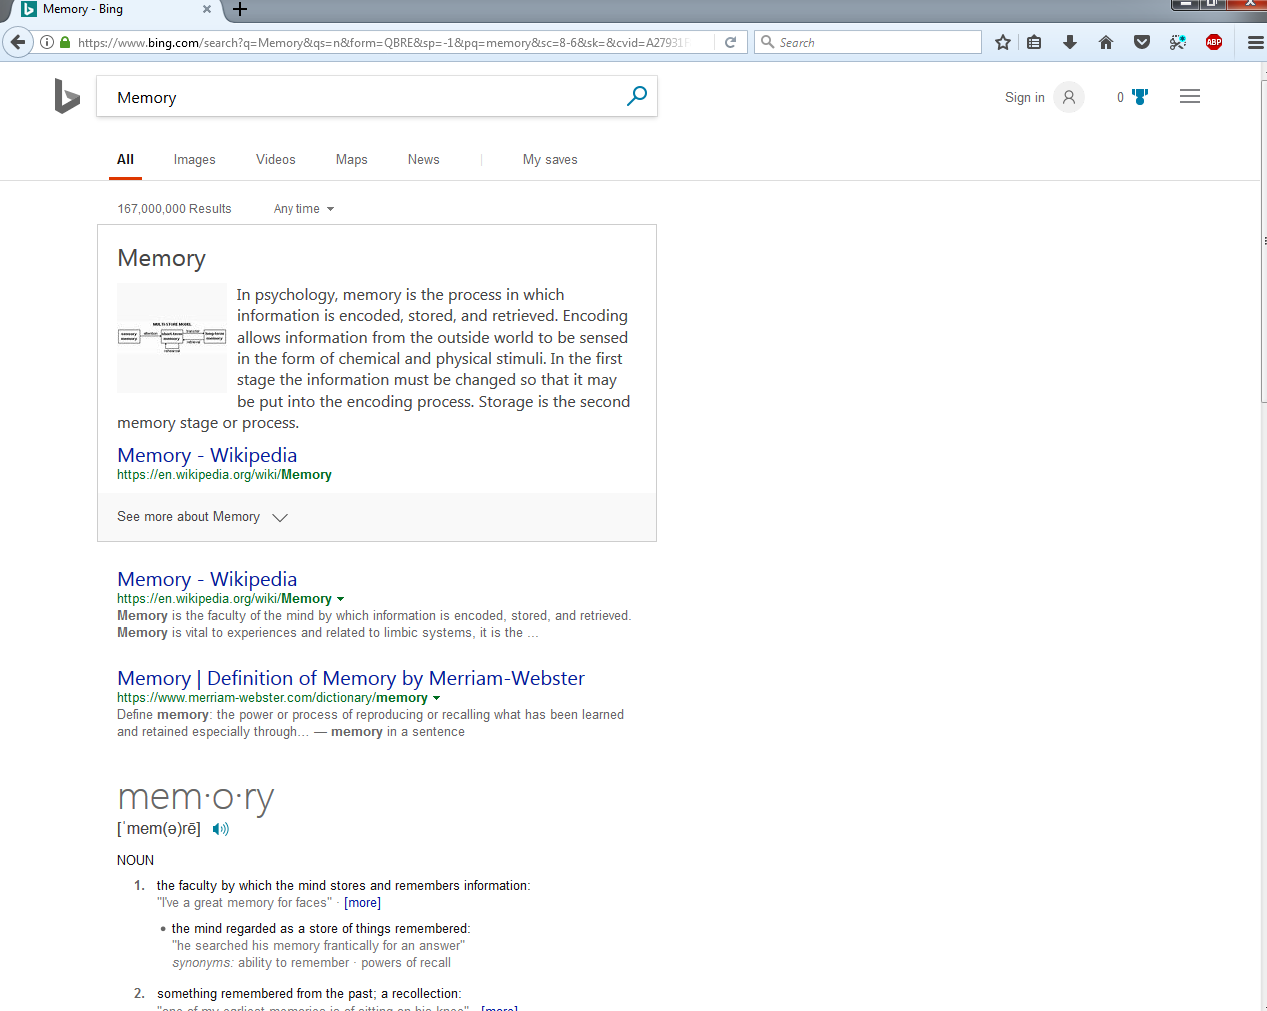
\includegraphics[scale=0.4]{Q1/MemoryBing.png}
\end{figure}

\pagebreak
Bing found about 3,220,000 results for the query ``Diesel Memory''.
\begin{figure}[h]
\caption{Query: Diesel Memory, Search Engine: Bing}
\centering
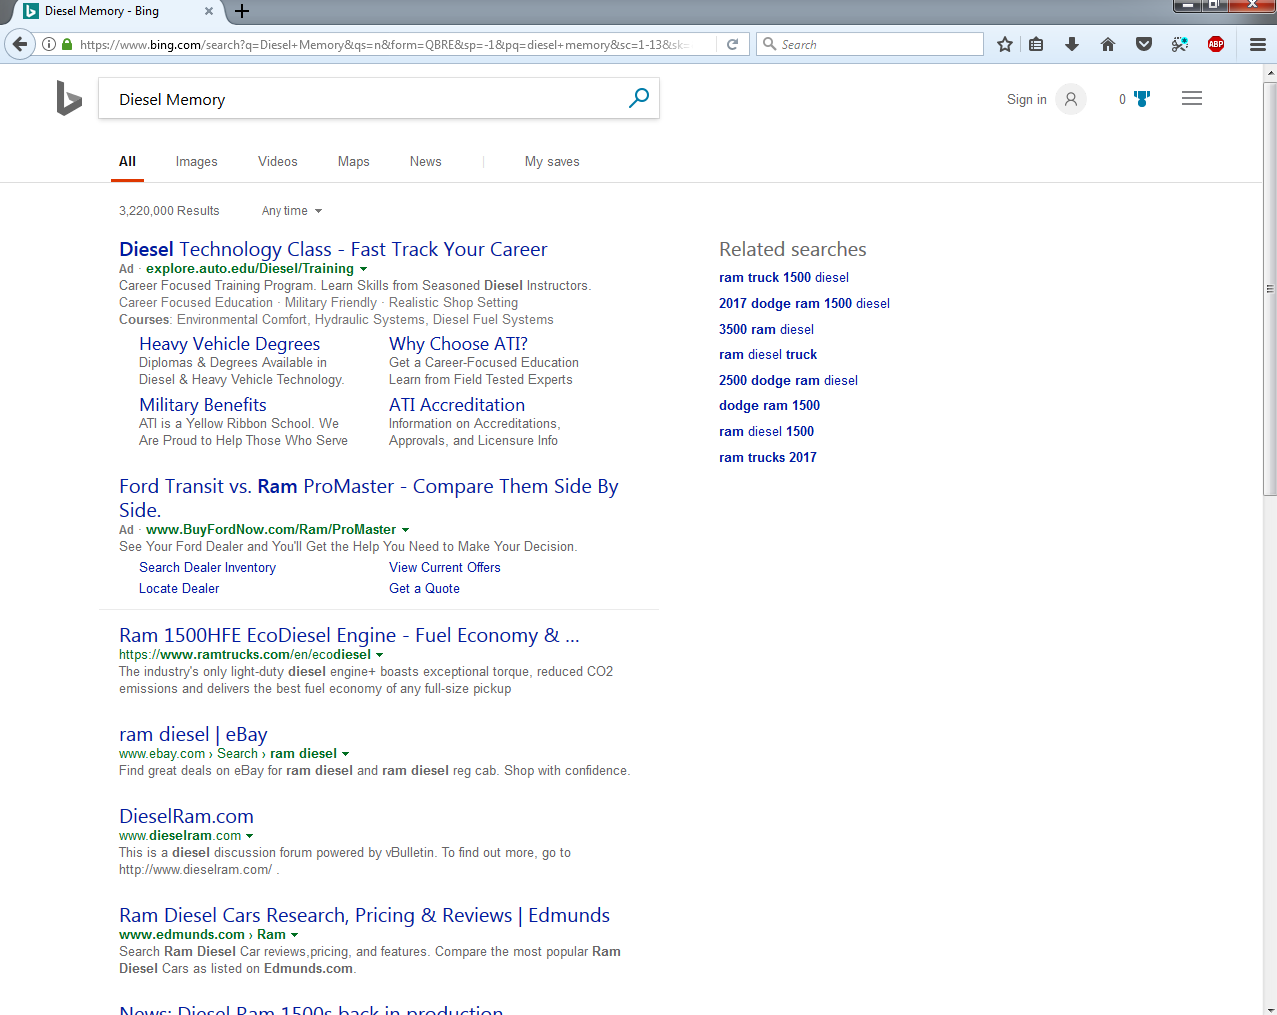
\includegraphics[scale=0.4]{Q1/DieselMemoryBing.png}
\end{figure}

Plugging the results in the formula gives the following:

$$N_{Bing} = \frac{183,000,000 \times 167,000,000}{3,220,000} = 9490993788.819876 \approx 9490993789
$$


\paragraph{2. Hairy Phone:}
I ran the second query ``Hairy Phone'' and found the following:

A. Google:

Google found about 106,000,000 results for the term ``Hairy''.

Google found about 1,410,000,000 results for the term ``Phone''.

Google found about 8,780,000 results for the query ``Hairy Phone''.

Plugging the results in the formula gives the following:

$$N_{google} = \frac{106,000,000 \times 1,410,000,000}{8,780,000} = 17022779043.28018 \approx 17022779043
$$

B. Bing:

Bing found about 292,000,000 results for the term ``Hairy''.

Bing found about 748,000,000 results for the term ``Phone''.

Bing found about 51,500,000 results for the query ``Hairy Phone''.

Plugging the results in the formula gives the following:

$$N_{Bing} = \frac{292,000,000 \times 748,000,000}{51,500,000} = 4241087378.640777 \approx 4241087379
$$

\paragraph{3. Computer Manifold:}
I ran the third query ``Computer Manifold'' and found the following:

A. Google:

Google found about 861,000,000 results for the term ``Computer''.

Google found about 21,500,000 results for the term ``Manifold''.

Google found about 6,470,000 results for the query ``Computer Manifold''.

Plugging the results in the formula gives the following:

$$N_{google} = \frac{861,000,000 \times 21,500,000}{6,470,000} = 2861128284.38949 \approx 2861128284
$$

B. Bing:

Bing found about 448,000,000 results for the term ``Computer''.

Bing found about 38,400,000 results for the term ``Manifold''.

Bing found about 35,100,000 results for the query ``Computer Manifold''.

Plugging the results in the formula gives the following:

$$N_{Bing} = \frac{448,000,000 \times 38,400,000}{35,100,000} = 490119658.1196581 \approx 490119658
$$

\paragraph{4. Electronic Lumber:}
I ran the forth query ``Electronic Lumber'' and found the following:

A. Google:

Google found about 1,010,000,000 results for the term ``Electronic''.

Google found about 43,300,000 results for the term ``Lumber''.

Google found about 5,720,000 results for the query ``Electronic Lumber''.

Plugging the results in the formula gives the following:

$$N_{google} = \frac{1,010,000,000 \times 43,300,000}{5,720,000} = 7645629370.629371 \approx 7645629371
$$

B. Bing:

Bing found about 289,000,000 results for the term ``Electronic''.

Bing found about 42,400,000 results for the term ``Lumber''.

Bing found about 244,000,000 results for the query ``Electronic Lumber''.

Plugging the results in the formula gives the following:

$$N_{Bing} = \frac{289,000,000 \times 42,400,000}{244,000,000} = 50219672.13114754 \approx 50219672
$$

The estimated number of indexed pages in Google as I found are:

2114878049

17022779043

2861128284

7645629371

It is clear that the estimates varied markedly, by few billions, for different queries. I assume that one of the reasons behind that is the difference in ``independence level'' of the two terms among different queries.

The estimated number of indexed pages in Bing as I found are:

9490993789

4241087379

490119658

50219672

The same inconsistency held for Bing. The estimates varied by few billions.


\section*{Question 2:}
Exercise 4.6:

Process five Wikipedia documents using the Porter stemmer and the Krovetz stemmer. Compare the number of stems produced and find 10 examples of differences in the stemming that could have an impact on ranking.

\section*{Answer:}

I have chosen the following documents from WikiSmall collection to process them using Porter and Krovetz stemmers.

Aakrosh\_(1998\_film).html

Aargau\_frank.html

Aaron\_Chalmers\_3ab5.html

Baba\_Budan\_67b5.html

Babs\_Fafunwa\_5f48.html

I wrote a simple python script PKstem.py to process the documents, stem the unique words in them, using Porter and Krovetz stemmers. The stemmers were not implemented from scratch because there are python libraries for both stemmers already.

\lstinputlisting[language=Python, breakatwhitespace=〈false), label=The content of PKstem.py, caption= The content of PKstem.py]{Q2/PKstem.py}

The program accepts the document(s) file name(s) as command line argument(s). It is possible to run the program and process all files at once, however, I ran each file separately.

After running the documents, I found the following results:

\textbf{Aakrosh\_(1998\_film).html}

Unique words: 229

Porter stems: 224

Krovetz stems: 227
 
\textbf{Aargau\_frank.html}

Unique words: 199

Porter stems: 193

Krovetz stems: 193

\textbf{Aaron\_Chalmers\_3ab5.html}

Unique words: 154

Porter stems: 149

Krovetz stems: 150

\textbf{Baba\_Budan\_67b5.html}

Unique words: 92

Porter stems: 90

Krovetz stems: 91

\textbf{Babs\_Fafunwa\_5f48.html}

Unique words: 239

Porter stems: 231

Krovetz stems: 235

This is a screen shot of running the program on the first file:



\begin{figure}[h]
\caption{Running PKstem.py}
\centering
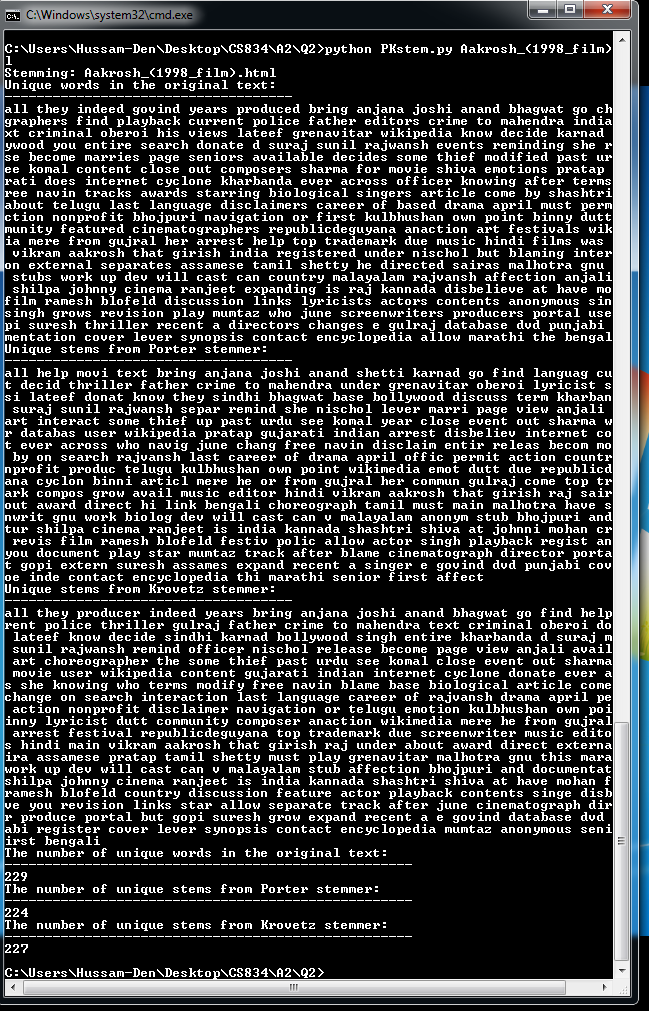
\includegraphics[scale=0.64]{Q2/PKstem.png}
\end{figure}

\pagebreak

I found the following examples of differences in the stemming that could have an impact on ranking:

\begin{longtable}{ |p{3cm}|p{3cm}|p{3cm}| } 
\hline
Original Text & Porter Stem & Krovetz Stem \\
 \hline 
 daily & daili & daily \\
 \hline
  changes & chang & change \\
 \hline
  academic & academ & academic \\
 \hline
  collaboration & collabor & collaboration \\
 \hline
  manchester & manchest & manchester \\
 \hline
  denominations & denomin & denomination \\
 \hline
  circulating & circul & circulate \\
 \hline
  article & articl & article \\
 \hline
  versus & versu & versus \\
 \hline
  association & associ & association \\
 \hline
\end{longtable}



\section*{Question 3:}
Exercise 4.8:

Find the 10 Wikipedia documents with the most inlinks. Show the collection of anchor text for those pages.

\section*{Answer:}

In order to find the 10 Wikipedia documents with the most inlinks, I created a small python script ``inlinks.py'' that extracts all links found in Wikipedia documents from WikiSmall collection. I stored the links as a key-value pair, where file name is the key and the link is the value. After grouping the links by their target, I counted them and sorted the files by the number of inlinks to find first 10  Wikipedia documents with the most inlinks.

\lstinputlisting[language=Python, breakatwhitespace=〈false), label=The content of inlinks.py, caption= The content of inlinks.py]{Q3/inlinks.py}

The program writes the result to a file ``output.txt''. This is a screen shot of the file:

\begin{figure}[h]
\caption{The output of inlinks.py}
\centering
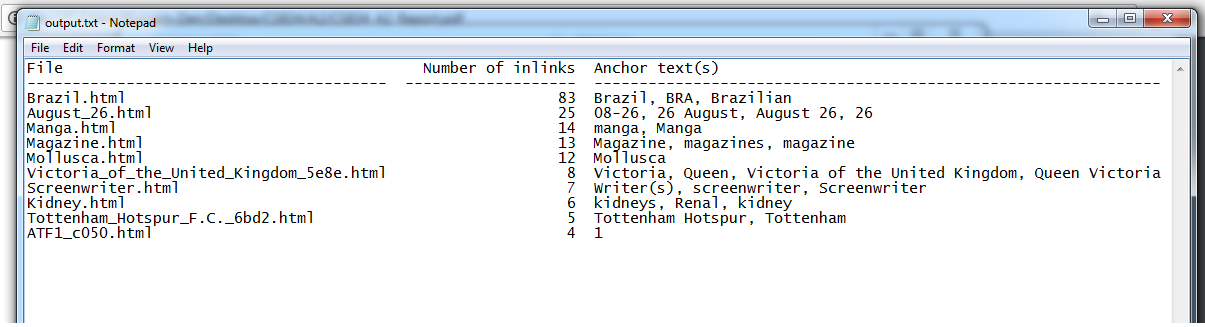
\includegraphics[scale=0.45]{Q3/inlinks.png}
\end{figure}


\section*{Question 4:}
Exercise 5.8: 

Write a program that can build a simple inverted index of a set of text documents. Each inverted list will contain the file names of the documents that contain that word.

Suppose the file A contains the text “the quick brown fox”, and file B contains “the slow blue fox”. The output of your program would be:

\% ./your-program A B

blue B

brown A

fox A B

quick A

slow B

the A B

\subsection*{Answer:}

To create an inverted index, we need to build a table of two columns. The first column contains the words that appear in the set of chosen documents, two in this case. The second column contains the documents in which the words appear.

I created a small python script ``inverted.py'' that accepts two command line arguments; these are the file names of the documents for which the inverted index will be built. The program stores the unique words in each document as a key-value pair where the document is the key and the words are the value. Swapping the key and the value will generate the inverted index we need. The output is printed on the screen and saved to the file ``output.txt''.

\lstinputlisting[language=Python, breakatwhitespace=〈false), label=The content of inverted.py, caption= The content of inverted.py]{Q4/inverted.py}

The files I chose to use to build the inverted index are taken from the WikiSmall collection. These files are:

Aakrosh\_(1998\_film).html

Babs\_Fafunwa\_5f48.html

\pagebreak

This is a screen shot of running the program:


\begin{figure}[h]
\caption{Running inverted.py}
\centering
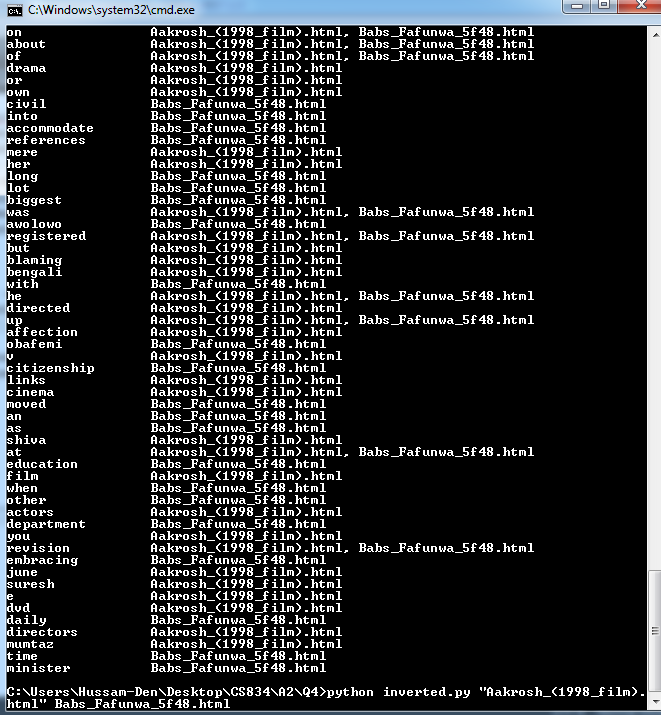
\includegraphics[scale=0.7]{Q4/inverted.png}
\end{figure}

\pagebreak

This is a screen shot of the output file ``output.txt'':

\begin{figure}[h]
\caption{output.txt screen shot}
\centering
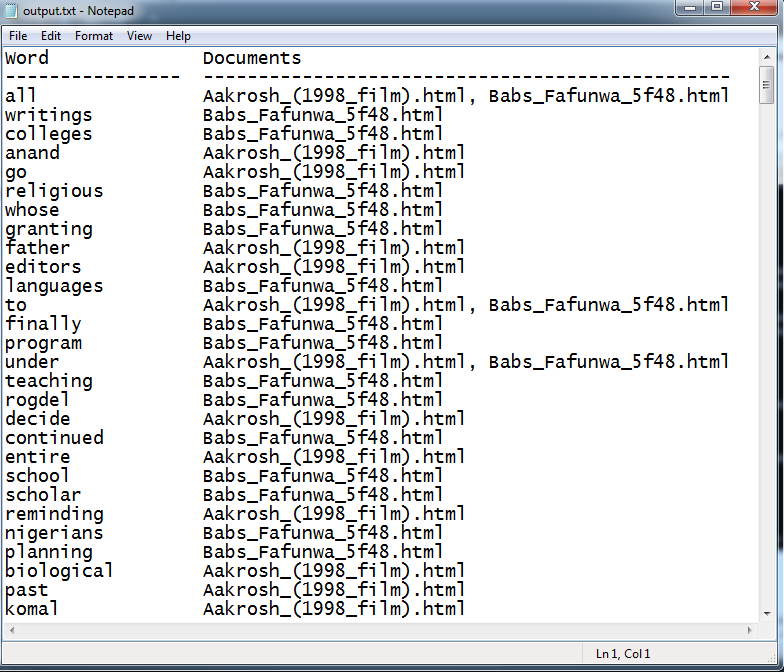
\includegraphics[scale=0.7]{Q4/output.png}
\end{figure}



\section*{Question 5:}
Exercise 5.10: 

Suppose a company develops a new unambiguous lossless compression scheme for 2-bit numbers called SuperShrink. Its developers claim that it will reduce the size of any sequence of 2-bit numbers by at least 1 bit. Prove that the developers are lying. More specifically, prove that either:

• SuperShrink never uses less space than an uncompressed encoding, or

• There is an input to SuperShrink such that the compressed version is larger than the uncompressed input

You can assume that each 2-bit input number is encoded separately.

\subsection*{Answer:}

We have 4 possible 2-bit numbers and 3 possible shorter bit sequences. Let's apply the pigeonhole principle, which states that if n items are put into m containers, with n > m, then at least one container must contain more than one item. This means that any mapping from 2-bit sequences to shorter sequences must have at least 2 sequences compressed to the same shorter sequence. Therefore, when trying to decompress this shorter sequence, mentioned above, it is impossible know which of the original 2-bit sequences it was compressed from.


\begin{thebibliography}{9}

\bibitem{} 
Stackoverflow. https://stackoverflow.com/questions/tagged/python.

\bibitem{} 
Sergey Brin and Larry Page. Google search engine. http://google.stanford.edu.

\bibitem{}
http://www.dba-oracle.com/oracle\_news/news\_ebay\_massive\_oracle.htm

\bibitem{}
https://www.wired.com/2012/01/amazon-dynamodb/

\bibitem{}
https://www.youtube.com/watch?v=a0OvgTfF8Pg

\bibitem{}
https://stackoverflow.com/questions/6526181/write-a-program-that-takes-text-as-input-and-produces-a-program-that-reproduces/6526266\#6526266

\bibitem{}
https://en.wikipedia.org/wiki/Pigeonhole\_principle


\end{thebibliography}


\end{document}